\pagebreak

\section{Experiments}\label{sec:experiments}
We put into action and assessed the outcomes of pose estimation for both synthetic and real data employing both the fundamental matrix and the trifocal tensor. \footnote{The MATLAB code to reproduce these experiments is available at the GitHub repository: \href{https://github.com/versi379/Two-View-Three-View-Pose-Estimation.git}{https://github.com/versi379/Two-View-Three-View-Pose-Estimation.git}.}

As for the \acs{FM}, we compute it both linearly (\acs{L-FM}) and through \acs{GH} (\acs{O-FM}), whereas for the \acs{TFT} we employ linear computation (\acs{L-TFT}) and apply \acs{GH} using minimal parametrizations proposed by Ressl (\acs{R-TFT}), Nordberg (\acs{N-TFT}), Faugeras \& Papadopoulo (\acs{FP-TFT}), and Ponce \& Hebert (\acs{PH-TFT}).

Additionally, we present the result obtained through \acs{BA}, which is initialised using any of the methods mentioned above. Remarkably, our experiments reveal that all initialisations yield nearly identical final poses post-minimization with \acs{BA} in the majority of cases..

\subsection{Synthetic Data}
We conducted trials on synthetic data to assess pose estimation using both the \acs{FM} and the \acs{TFT} across various configurations. The standard experimental setup consists of a collection of spatial points situated within a 400mm-sided cube centred at the world's origin, as shown in Figure (\ref{fig:syntheticScenes}). Points are projected onto three views, and Gaussian noise with a standard deviation of 1 pixel is applied to the image points, unless specified otherwise. The image dimensions are \( 1800 \times 1200 \) pixels, and since we assume a fixed focal length of 50mm, we represent a sensor size of \( 36mm \times 24mm \). All cameras are aligned to focus on the origin. Results are averaged over 30 simulations of data. \footnote{Synthetic trials are developed in the MATLAB script \textit{SyntheticExperiments.m} of the GitHub repository.}\\

\begin{figure}[h]
    \centering
    \subfigure[]{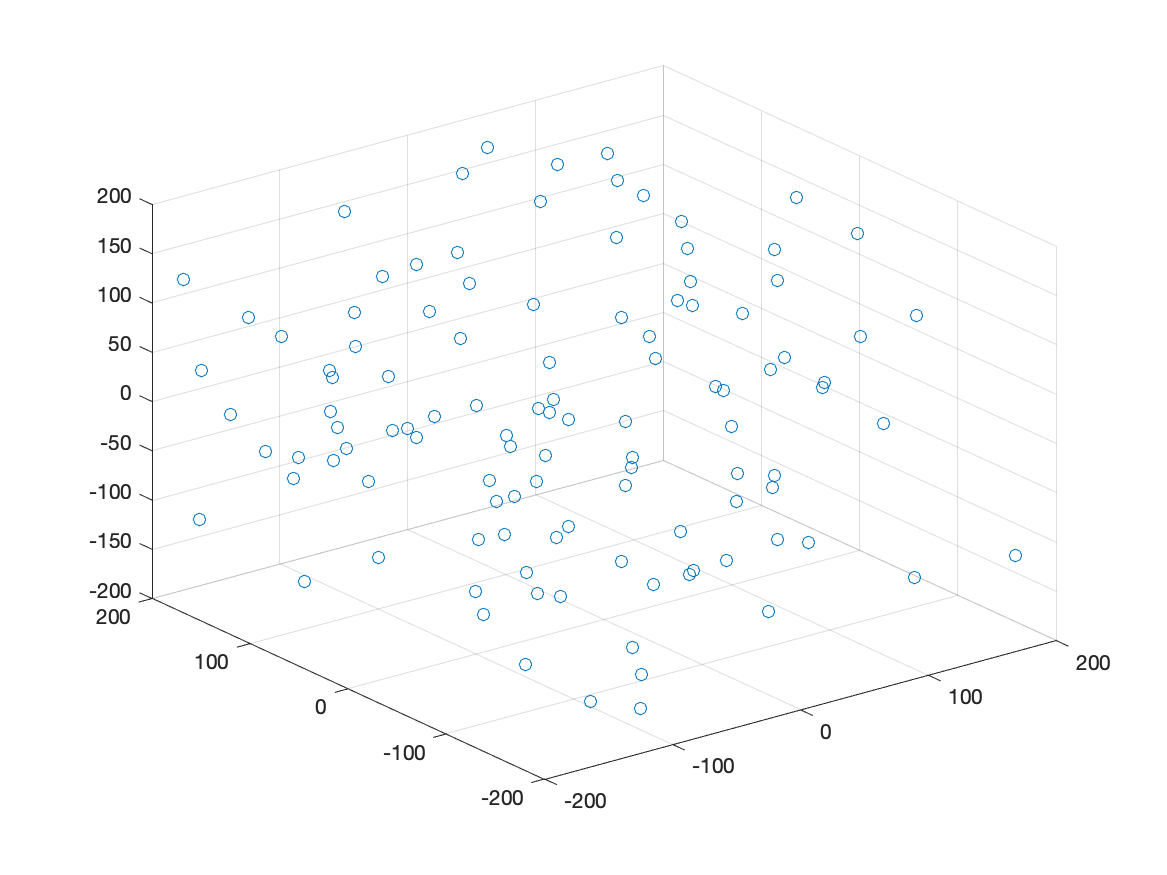
\includegraphics[width=0.33\textwidth]{Experiments/Synthetic/scene/IT1.png}} 
    \subfigure[]{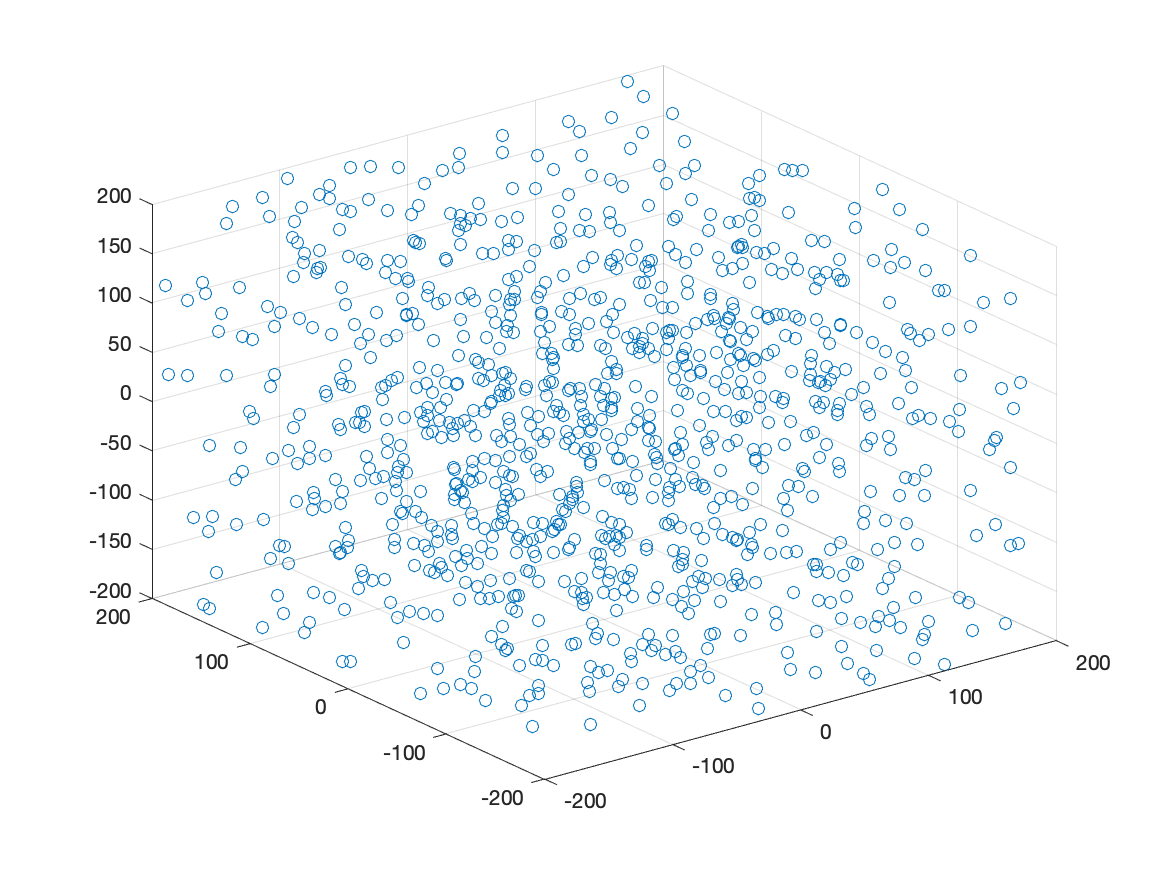
\includegraphics[width=0.33\textwidth]{Experiments/Synthetic/scene/IT10.png}}
    \\ 
    \subfigure[]{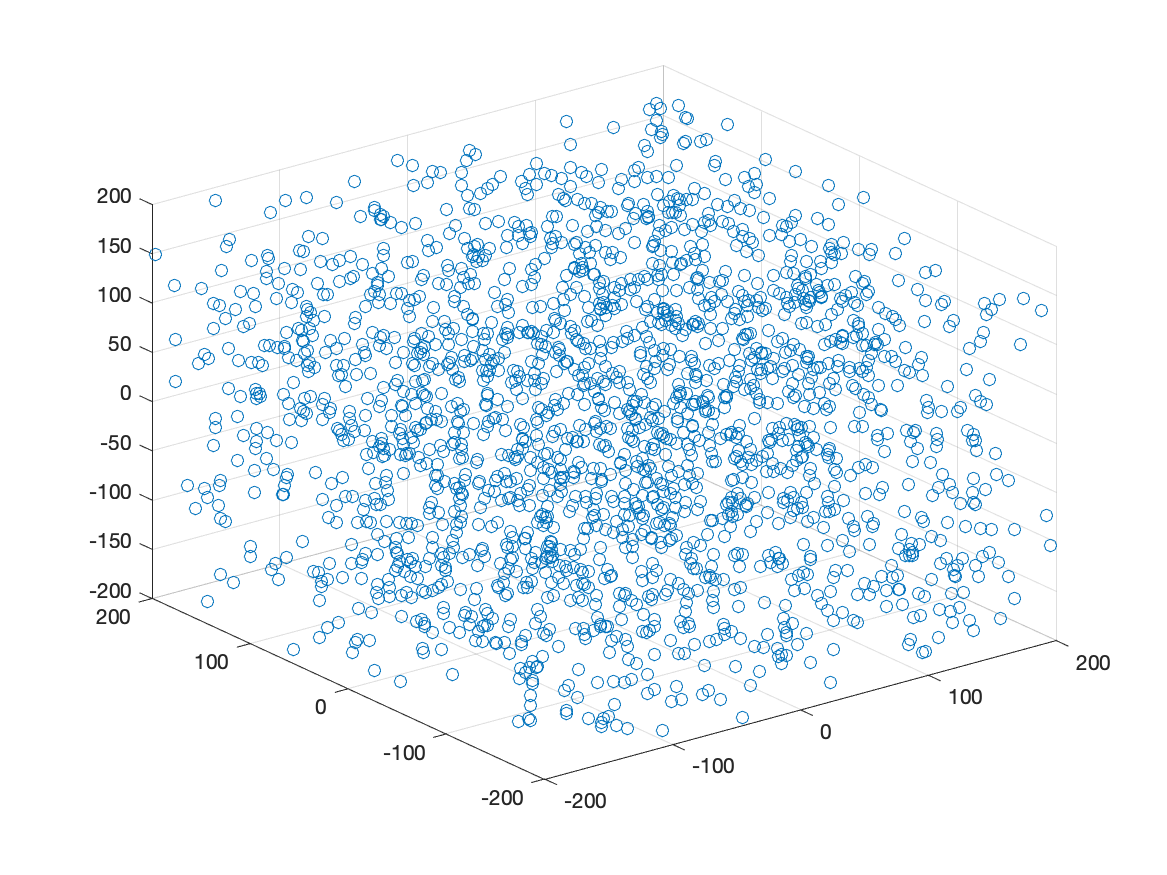
\includegraphics[width=0.33\textwidth]{Experiments/Synthetic/scene/IT20.png}}
    \subfigure[]{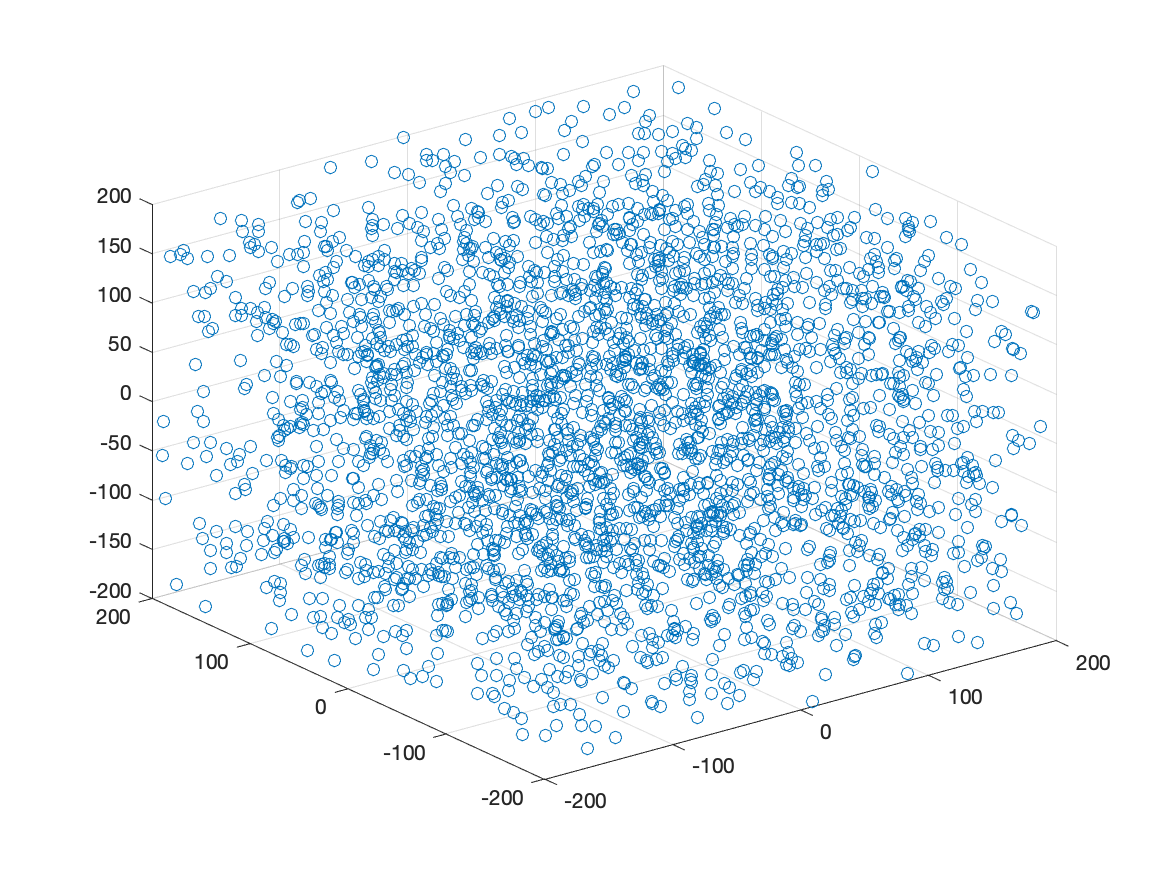
\includegraphics[width=0.33\textwidth]{Experiments/Synthetic/scene/IT30.png}}
    \caption[Synthetic Scene Setup]{Set of 3D points considered in the synthetic experiment setup: (a) 100 points simulation, (b) 1000 points simulation, (c) 2000 points simulation, (d) 3000 points simulation.}
    \label{fig:syntheticScenes}
\end{figure}

% to put image of synthetic points
\pagebreak

% Varying noise discussion
\subsubsection*{Metrics varying Noise}
Metrics before and after \acs{BA}, against Gaussian noise level added to the data points, are shown respectively in Figure (\ref{fig:initNoisePlot}) and Figure (\ref{fig:BANoisePlot}).

Initially, all methods show increasing reprojection, rotation, and translation errors as noise rises, with \acs{FP-TFT} and \acs{O-FM} demonstrating the lowest errors, indicating higher accuracy. Conversely, \acs{L-TFT} and \acs{R-TFT} exhibit higher errors, suggesting less robustness to noise. The number of iterations generally increases with noise, with \acs{N-TFT} requiring the most iterations, and \acs{L-TFT} showing the fastest computation times.

However, after \acs{BA}, all methods display significantly reduced errors and a linear increase with noise, indicating improved precision. The number of iterations and computational times remain relatively stable post-adjustment. Overall, these plots highlight a trade-off between accuracy and computational efficiency, with \acs{BA} enhancing performance across all methods, making them more precise and robust to noise.\\

% Varying focal length discussion
\subsubsection*{Metrics varying Focal Length}
Metrics before and after \acs{BA}, against varying focal length, are shown respectively in Figure (\ref{fig:initFocalPlot}) and Figure (\ref{fig:BAFocalPlot}).

Before \acs{BA}, the \acs{TFT} methods generally showed higher errors than the \acs{FM} methods. The \acs{L-TFT} had the highest initial errors in reprojection, rotation, and translation, while both the \acs{L-FM} and \acs{O-FM} performed better in initial estimates.

After applying \acs{BA}, the differences between parametrizations became less pronounced, especially for reprojection and rotation errors. The \acs{FP-TFT} and \acs{PH-TFT} methods seemed to perform consistently well across different metrics. The \acs{L-TFT}, while greatly improved, still showed higher errors and computation time in some cases compared to other parametrizations.\\

% Varying number of points discussion
\subsubsection*{Metrics varying Number of Points}
Metrics before and after \acs{BA}, against the number of points considered in the synthetic scene, are shown respectively in Figure (\ref{fig:initPointsPlot}) and Figure (\ref{fig:BAPointsPlot}).

Pre-\acs{BA} performances showed errors (reprojection, rotation, translation) being significantly higher for all methods, especially with a small number of points. The \acs{L-TFT} method generally showed the highest initial errors, whereas both the \acs{FM} methods often performed better in initial estimates.

Post-\acs{BA} performances showed error significantly reduced, with reprojection error decreasing from hundreds to less than 0.1 pixels, and rotation \& translation errors reduced to near-zero.

% Varying angle discussion
\subsubsection*{Metrics varying Camera Angle}
Metrics before and after Bundle Adjustment, against the varying angle among the three camera centers, are shown respectively in Figure (\ref{fig:initAnglePlot}) and Figure (\ref{fig:BAAnglePlot}).

Again, results after \acs{BA} are clearly more accurate with respect to the initial ones, with errors being almost null for all methods except \acs{N-TFT}, which showed peaks for certain angular values.

\begin{figure}[p]
	\centering
	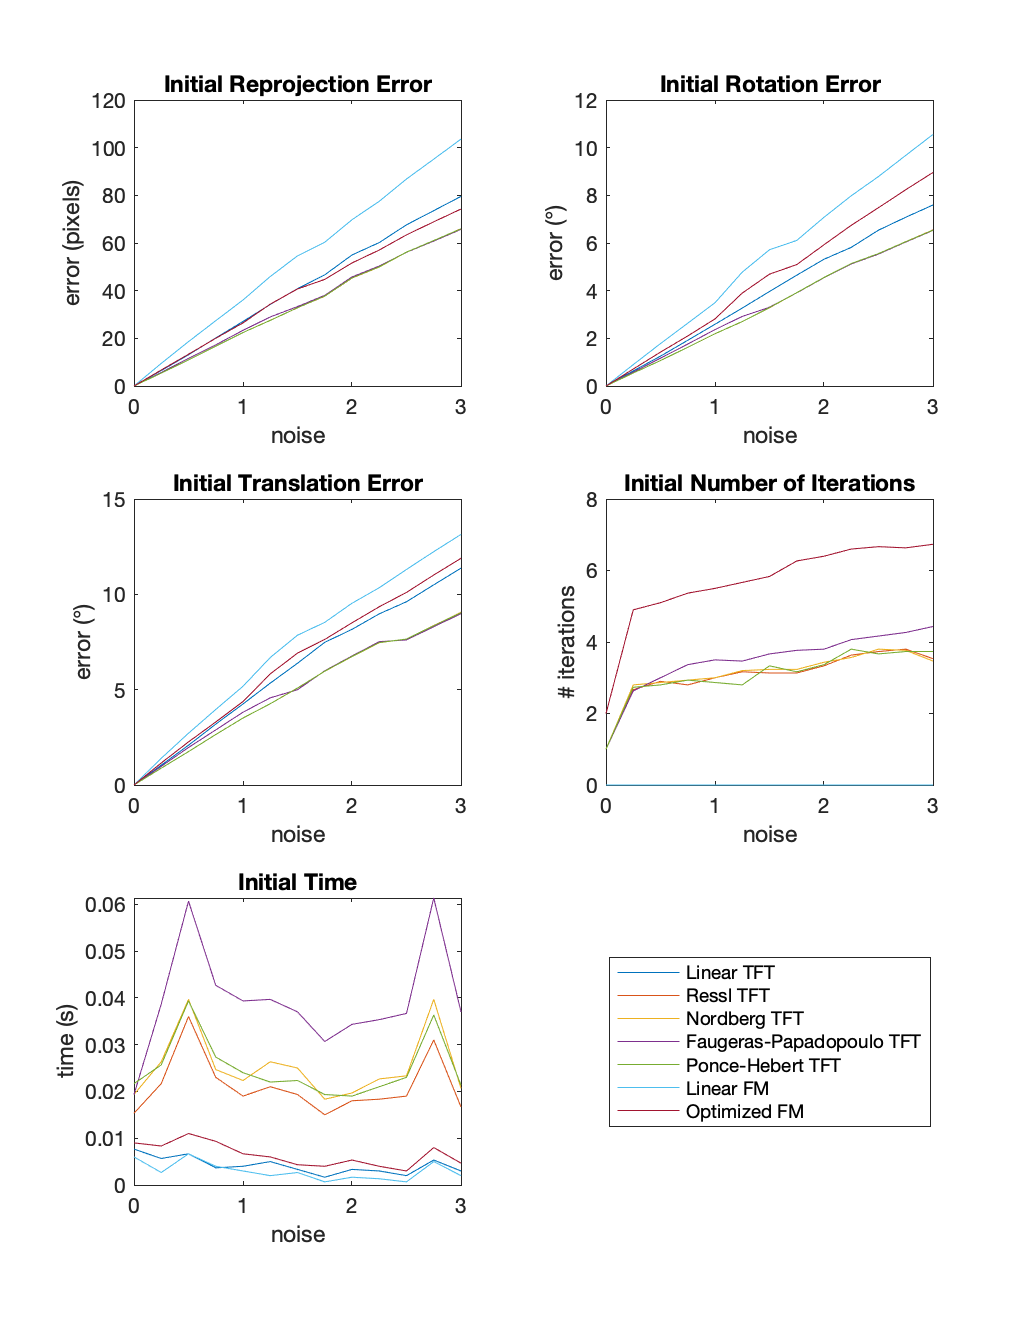
\includegraphics[width=1\textwidth]{Experiments/Synthetic/noise/INITnoisePlots.png}
	\caption[Synthetic Trial varying Gaussian Noise]{Initial reprojection error (top-left), rotation error (top-right), translation error (mid-left), number of iterations (mid-right), computational time (bottom-left); when varying the Gaussian noise added to the image points.}
	\label{fig:initNoisePlot}
\end{figure}

\begin{figure}[p]
	\centering
	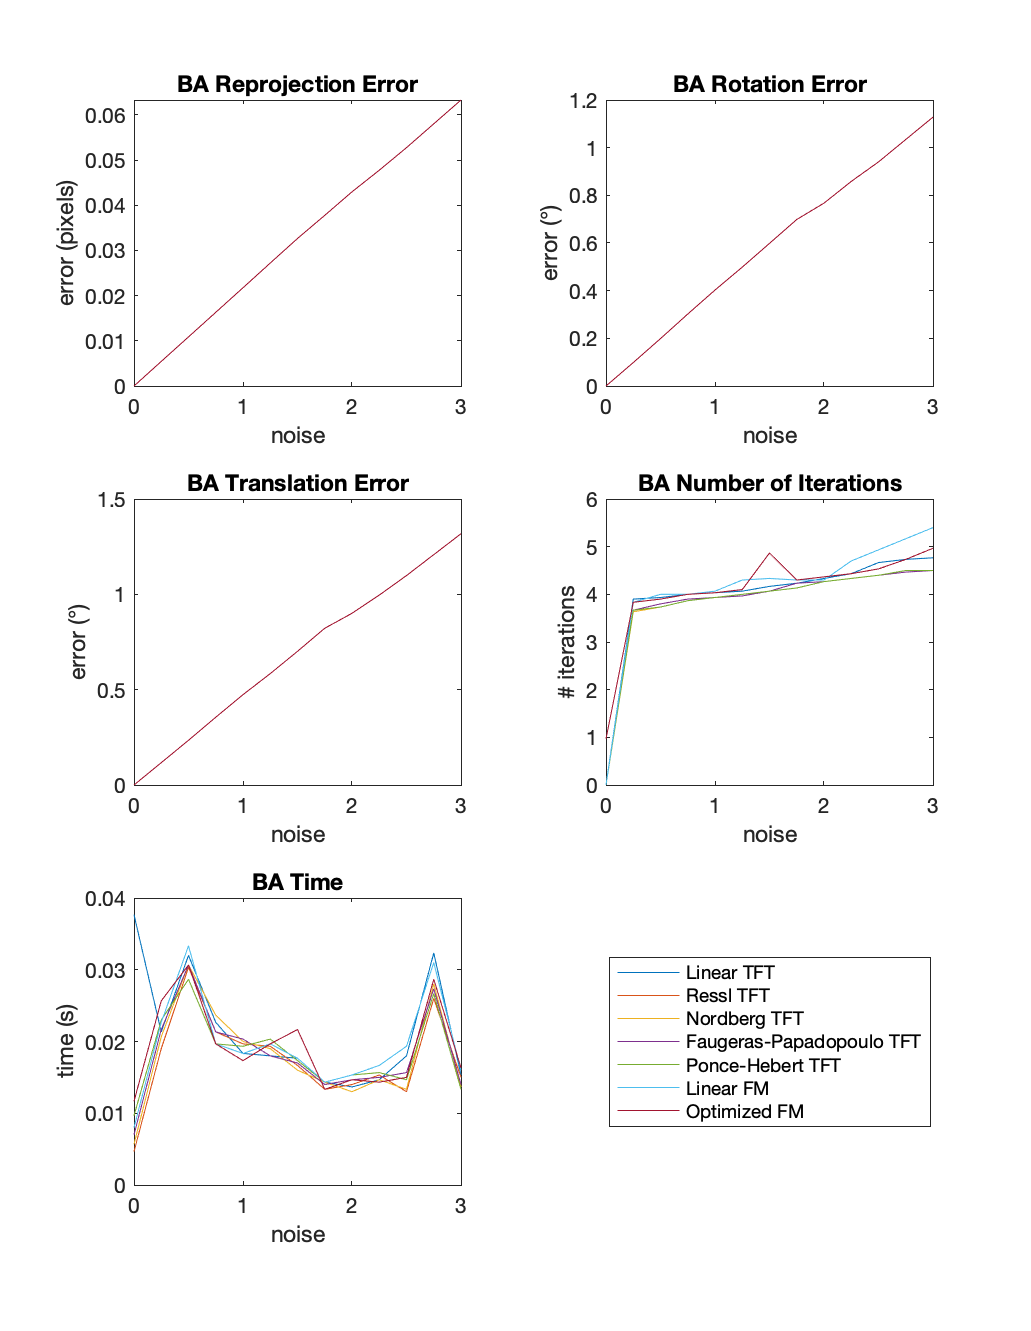
\includegraphics[width=1\textwidth]{Experiments/Synthetic/noise/BAnoisePlots.png}
	\caption[Synthetic Trial varying Gaussian Noise with \acs{BA}]{Reprojection error (top-left), rotation error (top-right), translation error (mid-left), number of iterations (mid-right), computational time (bottom-left) after \acs{BA}; when varying the Gaussian noise added to the image points.}
	\label{fig:BANoisePlot}
\end{figure}

\begin{figure}[p]
	\centering
	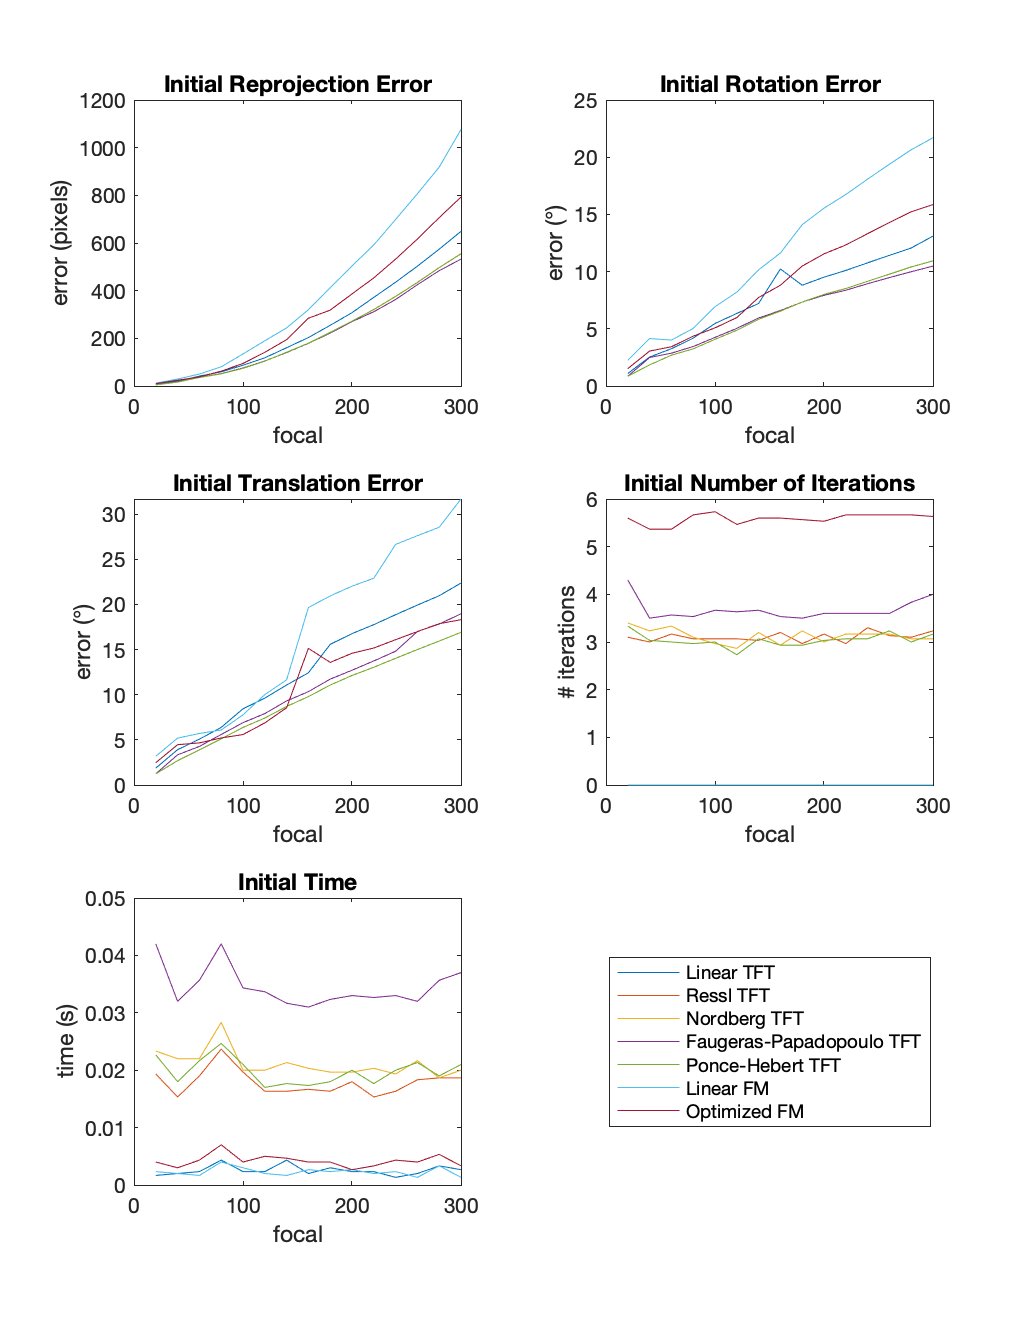
\includegraphics[width=1\textwidth]{Experiments/Synthetic/focal/INITfocalPlots.png}
	\caption[Synthetic Trial varying Focal Length]{Initial reprojection error (top-left), rotation error (top-right), translation error (mid-left), number of iterations (mid-right), computational time (bottom-left); when varying the focal length.}
	\label{fig:initFocalPlot}
\end{figure}

\begin{figure}[p]
	\centering
	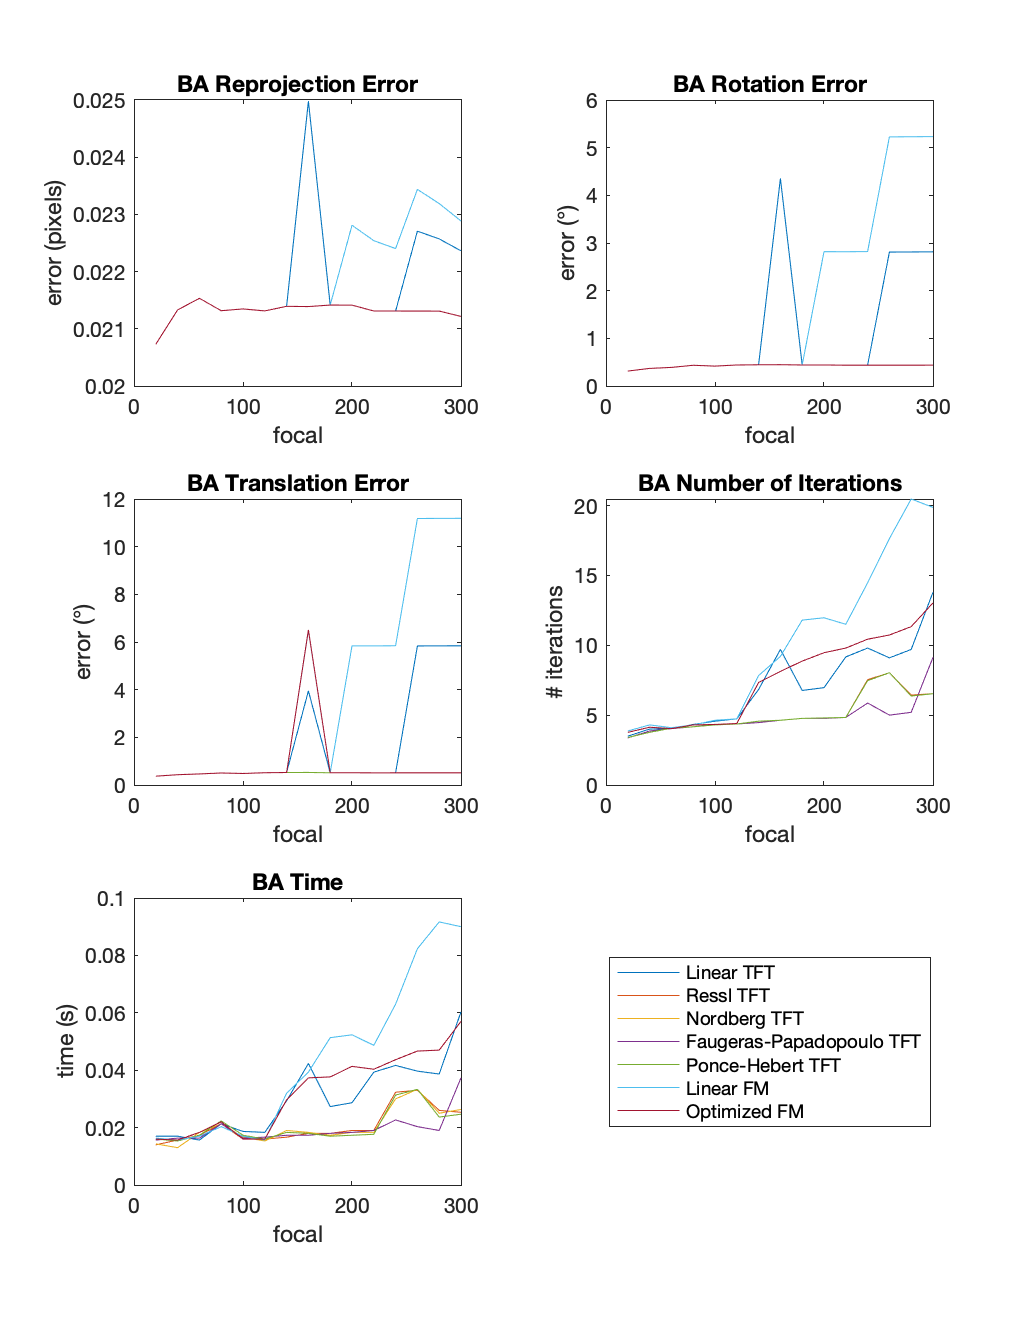
\includegraphics[width=1\textwidth]{Experiments/Synthetic/focal/BAfocalPlots.png}
	\caption[Synthetic Trial varying Focal Length with \acs{BA}]{Reprojection error (top-left), rotation error (top-right), translation error (mid-left), number of iterations (mid-right), computational time (bottom-left) after \acs{BA}; when varying the focal length.}
	\label{fig:BAFocalPlot}
\end{figure}

\begin{figure}[p]
	\centering
	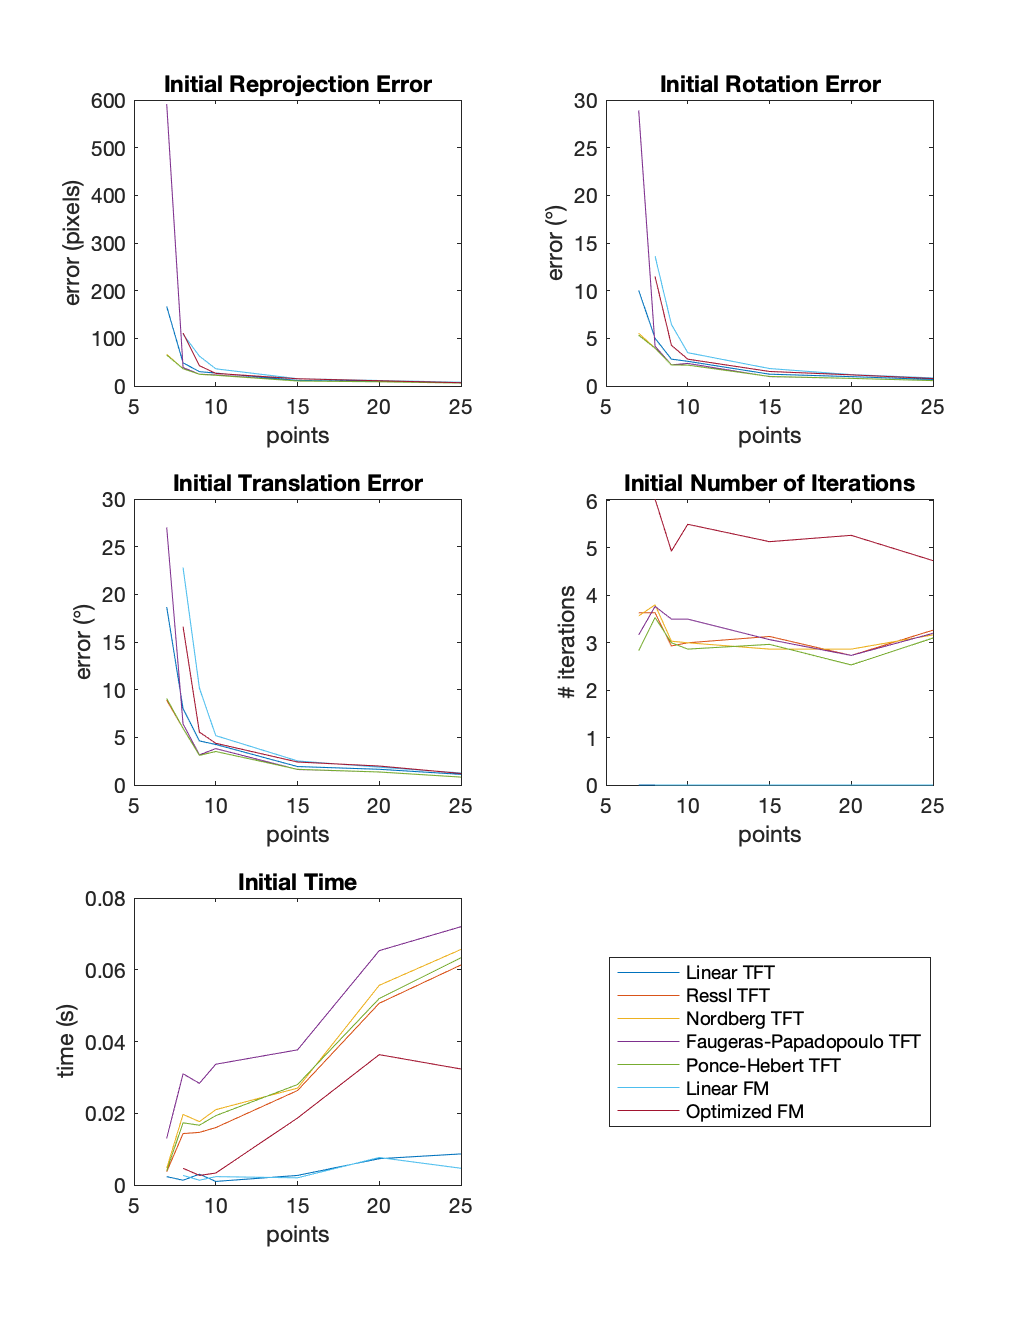
\includegraphics[width=1\textwidth]{Experiments/Synthetic/points/INITpointsPlots.png}
	\caption[Synthetic Trial varying Number of Image Points]{Initial reprojection error (top-left), rotation error (top-right), translation error (mid-left), number of iterations (mid-right), computational time (bottom-left); when varying the number of image points.}
	\label{fig:initPointsPlot}
\end{figure}

\begin{figure}[p]
	\centering
	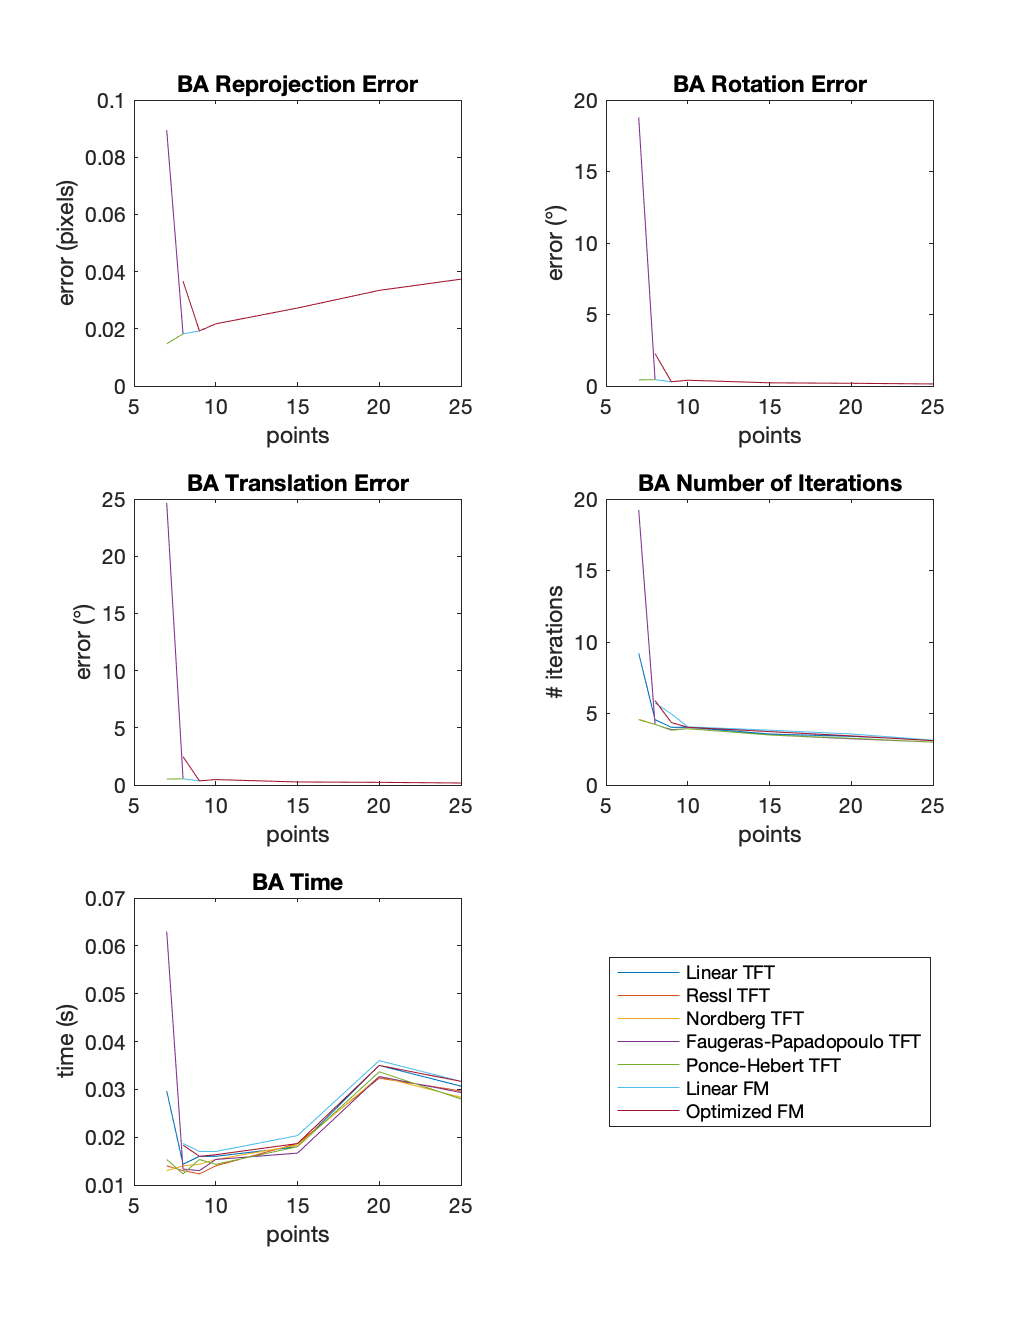
\includegraphics[width=1\textwidth]{Experiments/Synthetic/points/BApointsPlots.png}
	\caption[Synthetic Trial varying Number of Image Points with \acs{BA}]{Reprojection error (top-left), rotation error (top-right), translation error (mid-left), number of iterations (mid-right), computational time (bottom-left) after \acs{BA}; when varying the number of image points.}
	\label{fig:BAPointsPlot}
\end{figure}

\begin{figure}[p]
	\centering
	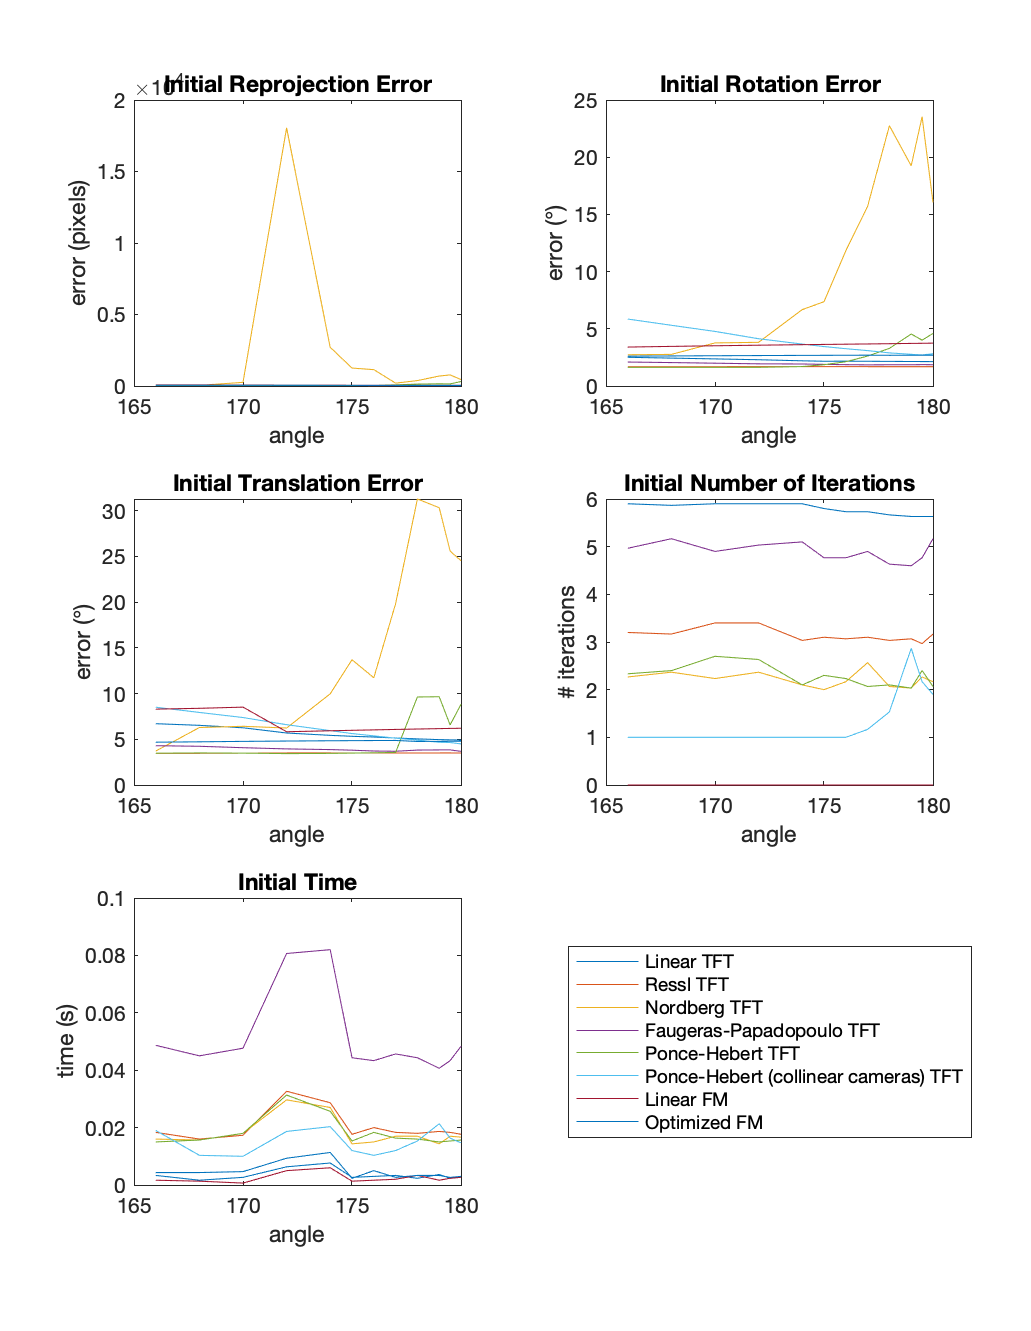
\includegraphics[width=1\textwidth]{Experiments/Synthetic/angle/INITanglePlots.png}
	\caption[Synthetic Trial varying Camera Centers Angle]{Initial reprojection error (top-left), rotation error (top-right), translation error (mid-left), number of iterations (mid-right), computational time (bottom-left); when varying the angle among the three camera centers.}
	\label{fig:initAnglePlot}
\end{figure}

\begin{figure}[p]
	\centering
	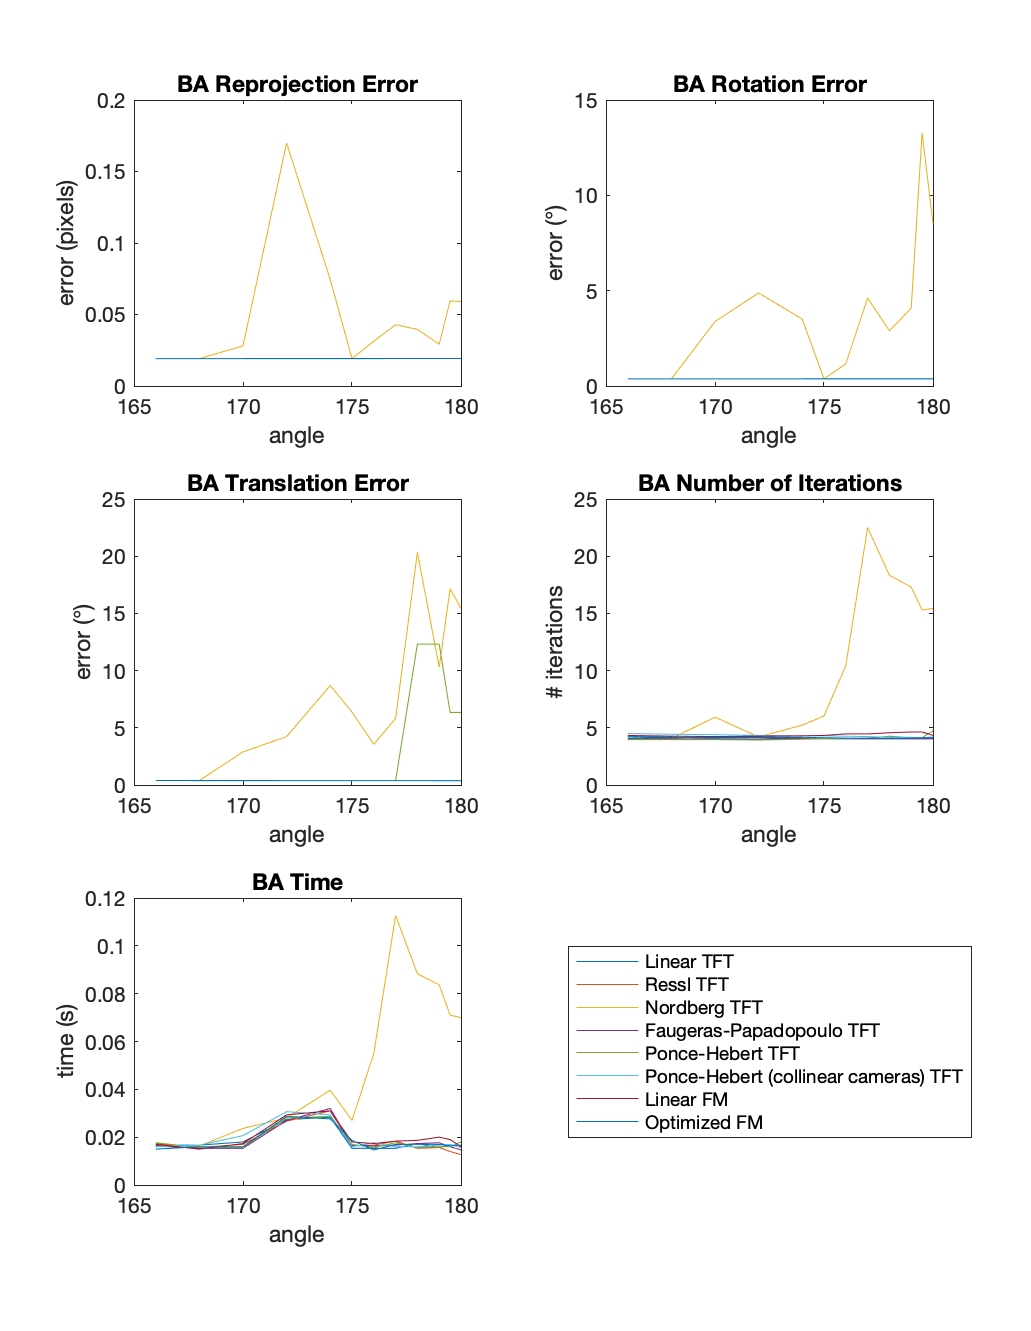
\includegraphics[width=1\textwidth]{Experiments/Synthetic/angle/BAanglePlots.png}
	\caption[Synthetic Trial varying Camera Centers Angle with \acs{BA}]{Reprojection error (top-left), rotation error (top-right), translation error (mid-left), number of iterations (mid-right), computational time (bottom-left) after \acs{BA}; when varying the angle among the three camera centers.}
	\label{fig:BAAnglePlot}
\end{figure}

\pagebreak

\subsection{Real Data}
In assessing the efficacy of these methods within real-world contexts, we opted to utilize scenes from the EPFL Dense Multi-View Stereo Dataset, presented in \cite{13-epfl-dataset}, provided by the CVLab at EPFL. \footnote{The EPFL Dense Multi-View Stereo Dataset, featuring the scenes utilized in our study, is readily accessible at the following location: \href{https://documents.epfl.ch/groups/c/cv/cvlab-unit/www/data/multiview/denseMVS.html}{https://documents.epfl.ch/groups/c/cv/cvlab-unit/www/data/multiview/denseMVS.html}.} \footnote{Real trials are developed in the MATLAB script \textit{RealExperiments.m} of the GitHub repository.}\\

Table (\ref{tab:fountainInit}) and (\ref{tab:fountainBA}) show metrics before and after \acs{BA} with respect to the \textit{fountain-P11} set of images from the dataset.

\begin{figure}[h]
    \centering
    \subfigure[]{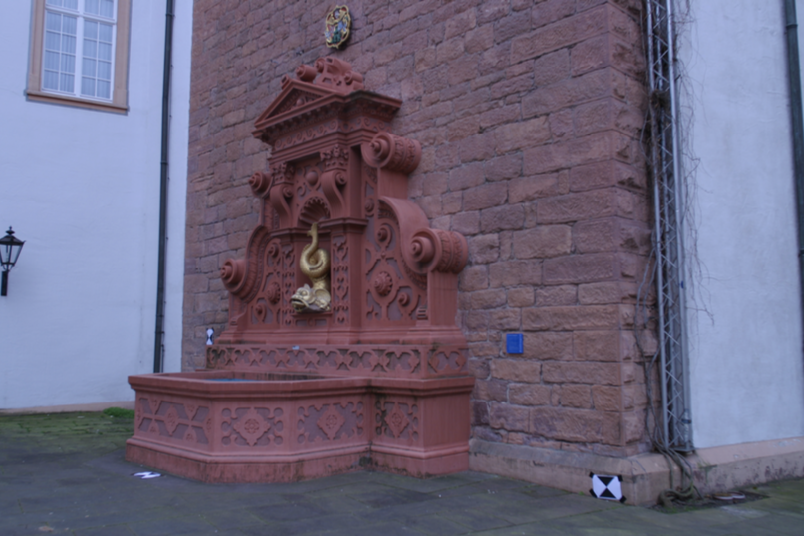
\includegraphics[width=0.30\textwidth]{Dataset/imgsReport/fountain1.png}} 
    \subfigure[]{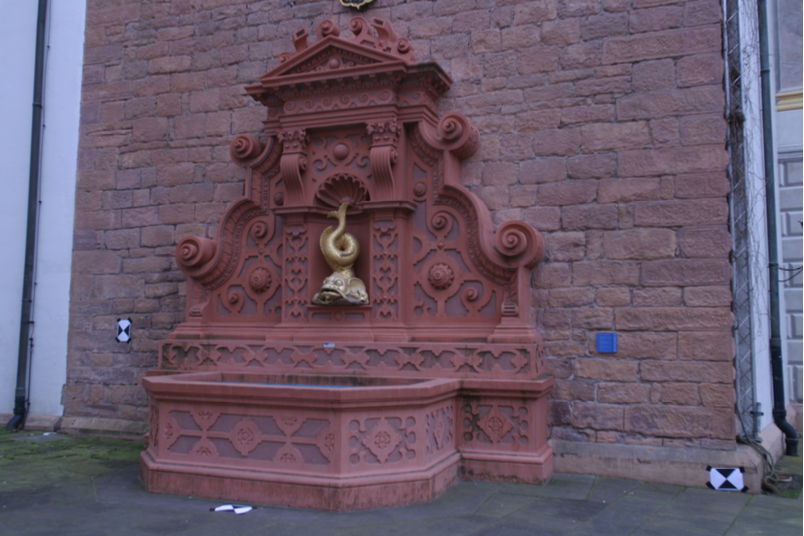
\includegraphics[width=0.30\textwidth]{Dataset/imgsReport/fountain2.png}} 
    \subfigure[]{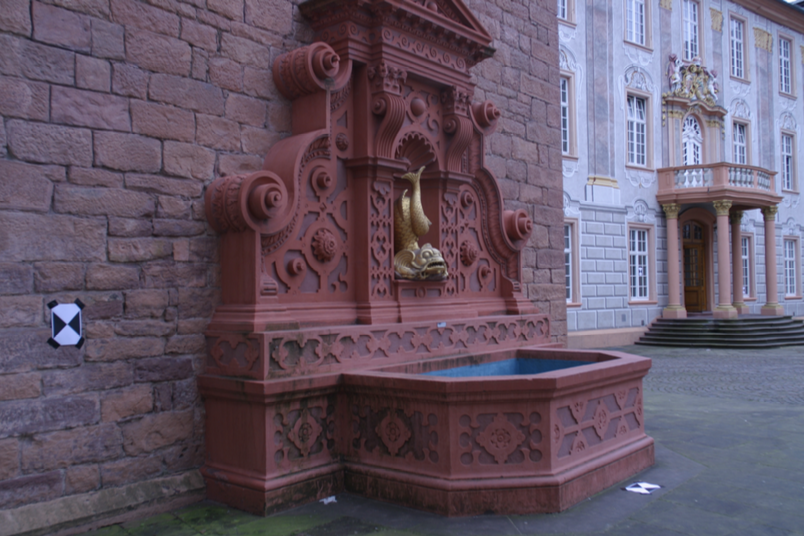
\includegraphics[width=0.30\textwidth]{Dataset/imgsReport/fountain3.png}}
    \caption[\textit{fountain-P11} Triplet]{Generic three-view triplet of images with respect to \textit{fountain-P11}. \cite{13-epfl-dataset}}
    \label{fig:fountainImage}
\end{figure}

\begin{table}[htbp]
  \centering
  \caption[\textit{fountain-P11} Initial Metrics]{Initial metrics with respect to the \textit{fountain-P11} set of images.}
  \label{tab:fountainInit}
  \begin{tabular}{|*{6}{c}|}
    \hline
     & repr. error (px) & R error ($^{\circ}$) & t error ($^{\circ}$) & \# iter. & time (s)\\
    \hline
    \acs{L-TFT} & 2.3953 & 0.1249 & 0.4048 & 0 & 0.0621 \\
    \acs{R-TFT} & 2.0474 & 0.1158 & 0.4003 & 2.8429 & 0.6400 \\
    \acs{N-TFT} & 2.1322 & 0.1334 & 0.4028 & 2.8000 & 0.6280 \\
    \acs{FP-TFT} & 2.3688 & 0.1187 & 0.4055 & 2.7714 & 0.6073 \\
    \acs{PH-TFT} & 2.0871 & 0.1167 & 0.4030 & 2.5857 & 0.5554 \\
    \acs{L-FM} & 1.9671 & 0.1149 & 0.3717 & 0 & 0.0273 \\
    \acs{O-FM} & 1.9530 & 0.1127 & 0.3658 & 4.9286 & 0.3209 \\
    \hline
  \end{tabular}
\end{table}

\begin{table}[htbp]
  \centering
  \caption[\textit{fountain-P11} Metrics with \acs{BA}]{Metrics after \acs{BA} with respect to the \textit{fountain-P11} set of images.}
  \label{tab:fountainBA}
  \begin{tabular}{|*{6}{c}|}
    \hline
     & repr. error (px) & R error ($^{\circ}$) & t error ($^{\circ}$) & \# iter. & time (s)\\
     \hline
    \acs{L-TFT} & 0.2814 & 0.0640 & 0.0743 & 3.8143 & 0.0743 \\
    \acs{R-TFT} & 0.2814 & 0.0640 & 0.0743 & 3.8286 & 0.0720 \\
    \acs{N-TFT} & 0.2814 & 0.0640 & 0.0743 & 3.8571 & 0.0716 \\
    \acs{FP-TFT} & 0.2814 & 0.0640 & 0.0743 & 3.8429 & 0.0723 \\
    \acs{PH-TFT} & 0.2814 & 0.0640 & 0.0743 & 3.8429 & 0.0743 \\
    \acs{L-FM} & 0.2814 & 0.0640 & 0.0743 & 3.7714 & 0.0816 \\
    \acs{O-FM} & 0.2814 & 0.0640 & 0.0743 & 3.8000 & 0.0784 \\
    \hline
  \end{tabular}
\end{table}

\pagebreak

Table (\ref{tab:HerzJesuInit}) and (\ref{tab:HerzJesuBA}) show metrics before and after \acs{BA} with respect to the \textit{Herz-Jesu-P8} set of images from the dataset.

\begin{figure}[h]
    \centering
    \subfigure[]{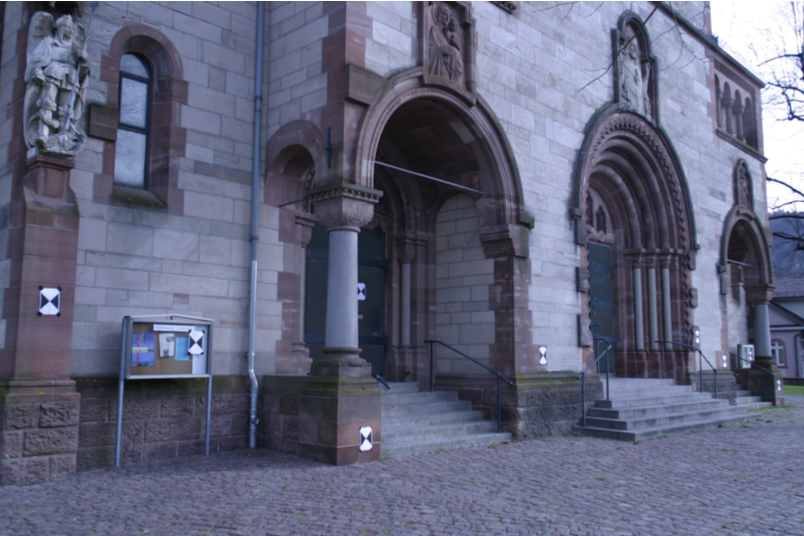
\includegraphics[width=0.30\textwidth]{Dataset/imgsReport/herzjesu1.png}} 
    \subfigure[]{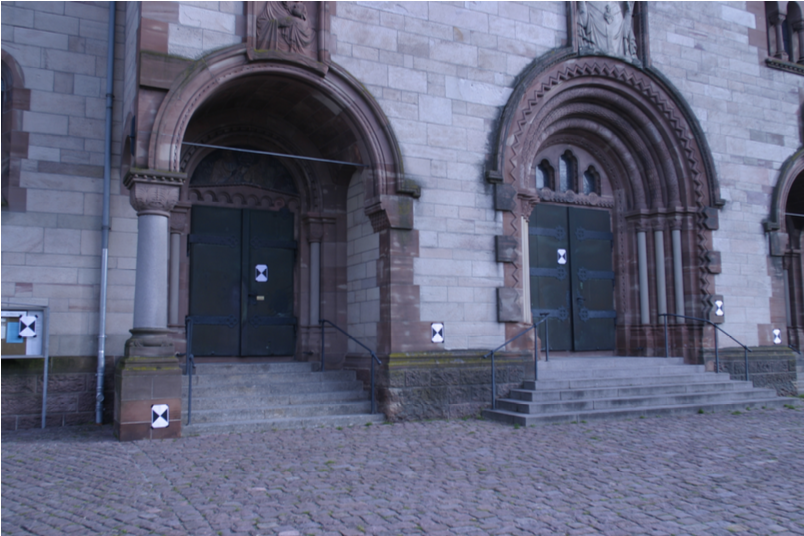
\includegraphics[width=0.30\textwidth]{Dataset/imgsReport/herzjesu2.png}} 
    \subfigure[]{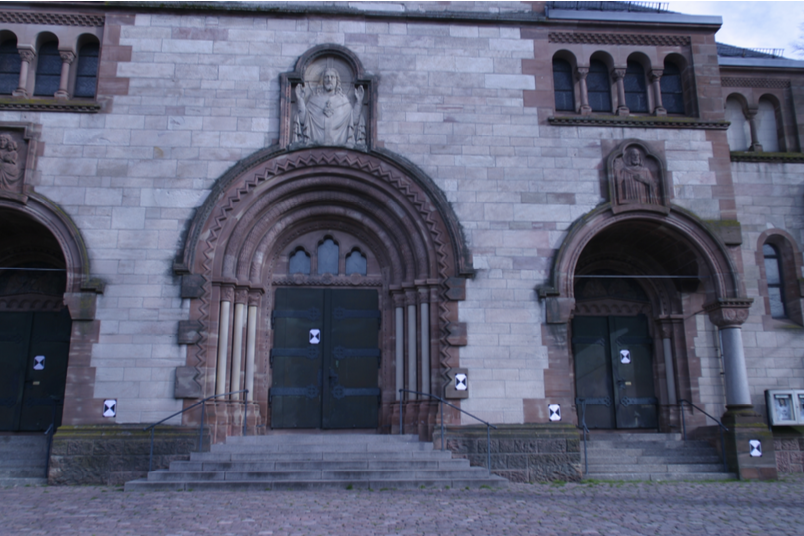
\includegraphics[width=0.30\textwidth]{Dataset/imgsReport/herzjesu3.png}}
    \caption[\textit{Herz-Jesu-P8} Triplet]{Generic three-view triplet of images with respect to \textit{Herz-Jesu-P8}. \cite{13-epfl-dataset}}
    \label{fig:herzjesuImage}
\end{figure}

\begin{table}[htbp]
  \centering
  \caption[\textit{Herz-Jesu-P8} Initial Metrics]{Initial metrics with respect to the \textit{Herz-Jesu-P8} set of images.}
  \label{tab:HerzJesuInit}
  \begin{tabular}{|*{6}{c}|}
    \hline
     & repr. error (px) & R error ($^{\circ}$) & t error ($^{\circ}$) & \# iter. & time (s)\\
    \hline
    \acs{L-TFT} & 4.8062 & 0.4589 & 0.8707 & 0 & 0.0506 \\
    \acs{R-TFT} & 3.4792 & 0.3966 & 0.6677 & 2.7800 & 0.4904 \\
    \acs{N-TFT} & 4.0656 & 0.5252 & 0.6917 & 2.6600 & 0.4816 \\
    \acs{FP-TFT} & 4.5006 & 0.4459 & 0.8324 & 3.4400 & 0.5452 \\
    \acs{PH-TFT} & 4.5293 & 0.4261 & 0.6682 & 2.3000 & 0.4116 \\
    \acs{L-FM} & 3.7624 & 0.4142 & 0.7725 & 0 & 0.0224 \\
    \acs{O-FM} & 3.6503 & 0.4196 & 0.7654 & 5.6600 & 0.2906 \\
    \hline
  \end{tabular}
\end{table}

\begin{table}[htbp]
  \centering
  \caption[\textit{Herz-Jesu-P8} Metrics with \acs{BA}]{Metrics after \acs{BA} with respect to the \textit{Herz-Jesu-P8} set of images.}
  \label{tab:HerzJesuBA}
  \begin{tabular}{|*{6}{c}|}
    \hline
     & repr. error (px) & R error ($^{\circ}$) & t error ($^{\circ}$) & \# iter. & time (s)\\
    \hline
    \acs{L-TFT} & 0.3719 & 0.0635 & 0.0682 & 4.0600 & 0.0792 \\
    \acs{R-TFT} & 0.3719 & 0.0635 & 0.0682 & 4.0000 & 0.0674 \\
    \acs{N-TFT} & 0.3719 & 0.0635 & 0.0682 & 4.0400 & 0.0690 \\
    \acs{FP-TFT} & 0.3719 & 0.0635 & 0.0682 & 4.0600 & 0.0680 \\
    \acs{PH-TFT} & 0.3719 & 0.0635 & 0.0682 & 4.0000 & 0.0664 \\
    \acs{L-FM} & 0.3719 & 0.0635 & 0.0682 & 4.0000 & 0.0718 \\
    \acs{O-FM} & 0.3719 & 0.0635 & 0.0682 & 4.0200 & 0.0724 \\
    \hline
  \end{tabular}
\end{table}

\pagebreak

Table (\ref{tab:entryInit}) and (\ref{tab:entryBA}) show metrics before and after \acs{BA} with respect to the \textit{entry-P10} set of images from the dataset.

\begin{figure}[h]
    \centering
    \subfigure[]{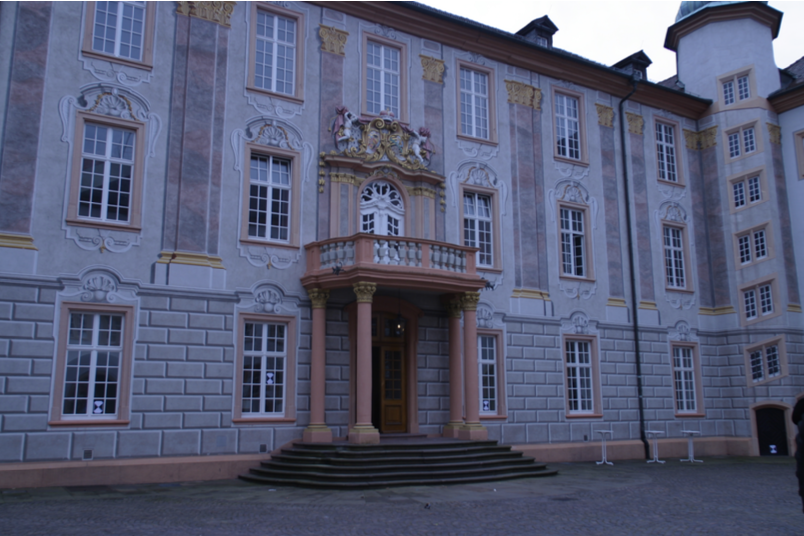
\includegraphics[width=0.30\textwidth]{Dataset/imgsReport/entry1.png}} 
    \subfigure[]{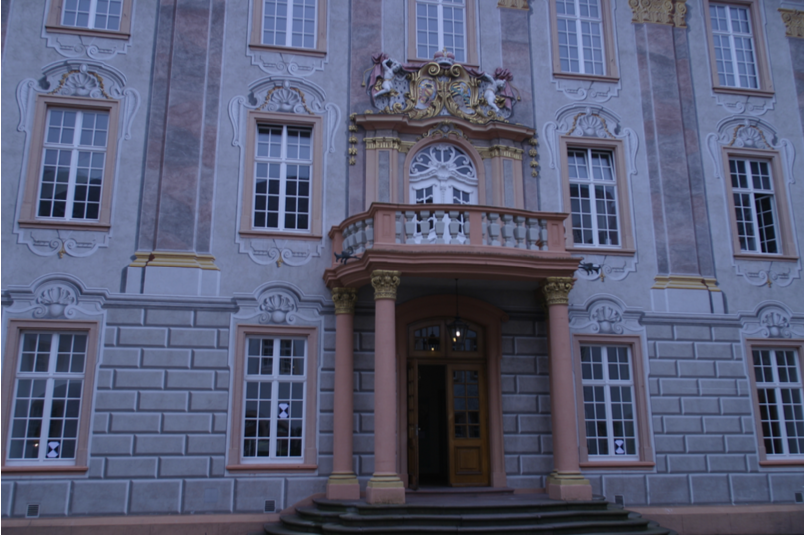
\includegraphics[width=0.30\textwidth]{Dataset/imgsReport/entry2.png}} 
    \subfigure[]{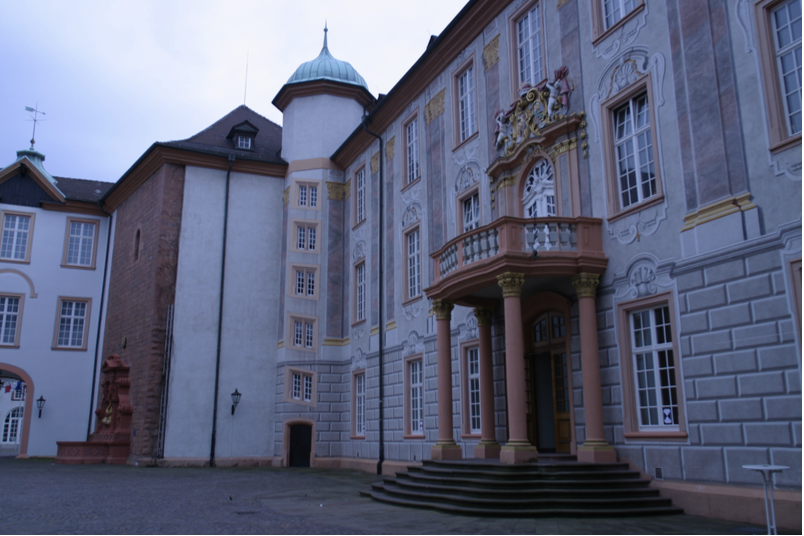
\includegraphics[width=0.30\textwidth]{Dataset/imgsReport/entry3.png}}
    \caption[\textit{entry-P10} Triplet]{Generic three-view triplet of images with respect to \textit{entry-P10}. \cite{13-epfl-dataset}}
    \label{fig:entryImage}
\end{figure}

\begin{table}[htbp]
  \centering
  \caption[\textit{entry-P10} Initial Metrics]{Initial metrics with respect to the \textit{entry-P10} set of images.}
  \label{tab:entryInit}
  \begin{tabular}{|*{6}{c}|}
    \hline
     & repr. error (px) & R error ($^{\circ}$) & t error ($^{\circ}$) & \# iter. & time (s)\\
    \hline
    \acs{L-TFT} & 3.8006 & 0.4144 & 0.8582 & 0 & 0.0572 \\
    \acs{R-TFT} & 3.1021 & 0.3872 & 0.6520 & 2.8200 & 0.5023 \\
    \acs{N-TFT} & 3.4590 & 0.4812 & 0.6833 & 2.7800 & 0.5144 \\
    \acs{FP-TFT} & 3.4480 & 0.4310 & 0.8246 & 3.5200 & 0.6340 \\
    \acs{PH-TFT} & 3.5078 & 0.4129 & 0.6619 & 2.4000 & 0.4389 \\
    \acs{L-FM} & 3.6451 & 0.4075 & 0.7103 & 0 & 0.0388 \\
    \acs{O-FM} & 3.6054 & 0.4018 & 0.7578 & 5.6800 & 0.3476 \\
    \hline
  \end{tabular}
\end{table}

\begin{table}[htbp]
  \centering
  \caption[\textit{entry-P10} Metrics with \acs{BA}]{Metrics after \acs{BA} with respect to the \textit{entry-P10} set of images.}
  \label{tab:entryBA}
  \begin{tabular}{|*{6}{c}|}
    \hline
     & repr. error (px) & R error ($^{\circ}$) & t error ($^{\circ}$) & \# iter. & time (s)\\
    \hline
    \acs{L-TFT} & 0.3479 & 0.0581 & 0.0634 & 4.0153 & 0.0811 \\
    \acs{R-TFT} & 0.3479 & 0.0581 & 0.0634 & 4.0242 & 0.0682 \\
    \acs{N-TFT} & 0.3479 & 0.0581 & 0.0634 & 4.0167 & 0.0708 \\
    \acs{FP-TFT} & 0.3479 & 0.0581 & 0.0634 & 4.0271 & 0.0714 \\
    \acs{PH-TFT} & 0.3479 & 0.0581 & 0.0634 & 4.0015 & 0.0679 \\
    \acs{L-FM} & 0.3479 & 0.0581 & 0.0634 & 3.9920 & 0.0734 \\
    \acs{O-FM} & 0.3479 & 0.0581 & 0.0634 & 4.0030 & 0.0751 \\
    \hline
  \end{tabular}
\end{table}

\pagebreak

Table (\ref{tab:castleInit}) and (\ref{tab:castleBA}) show metrics before and after \acs{BA} with respect to the \textit{castle-P19} set of images from the dataset.

\begin{figure}[h]
    \centering
    \subfigure[]{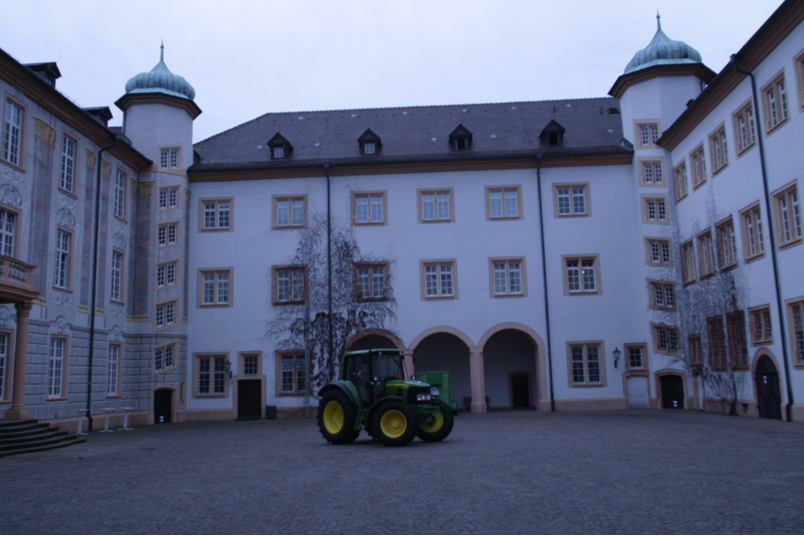
\includegraphics[width=0.30\textwidth]{Dataset/imgsReport/castle1.png}} 
    \subfigure[]{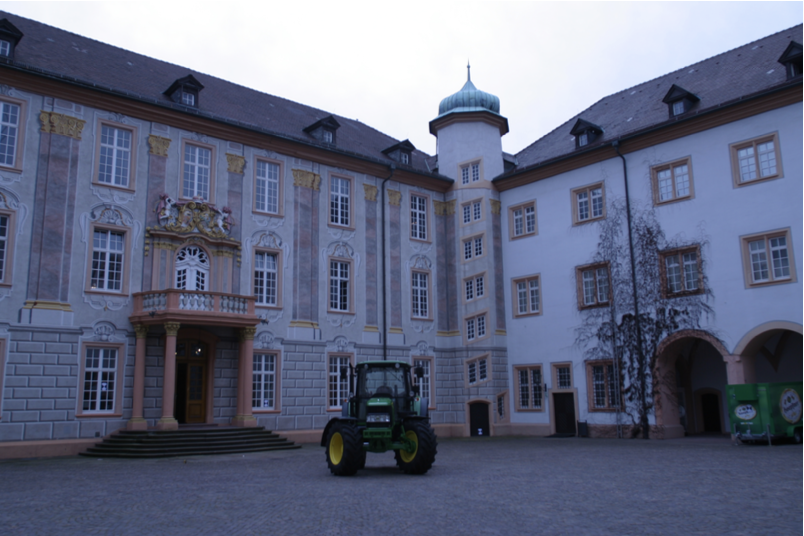
\includegraphics[width=0.30\textwidth]{Dataset/imgsReport/castle2.png}} 
    \subfigure[]{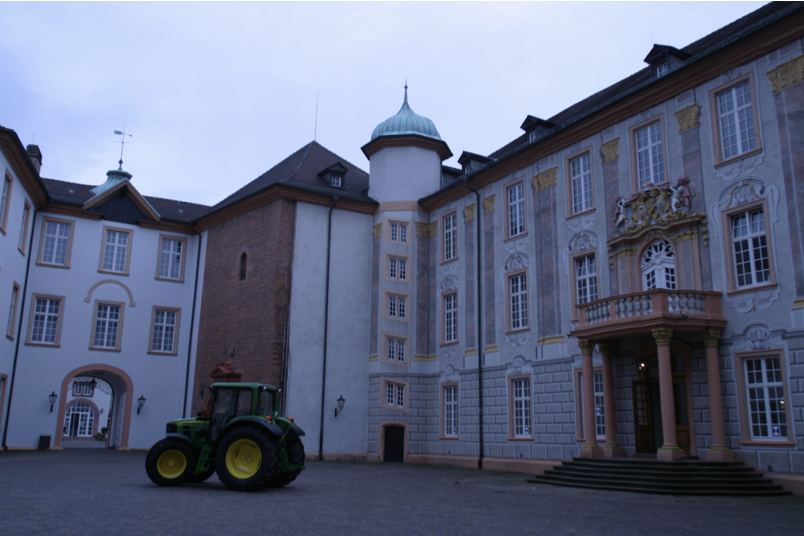
\includegraphics[width=0.30\textwidth]{Dataset/imgsReport/castle3.png}}
    \caption[\textit{castle-P19} Triplet]{Generic three-view triplet of images with respect to \textit{castle-P19}. \cite{13-epfl-dataset}}
    \label{fig:castleImage}
\end{figure}

\begin{table}[htbp]
  \centering
  \caption[\textit{castle-P19} Initial Metrics]{Initial metrics with respect to the \textit{castle-P19} set of images.}
  \label{tab:castleInit}
  \begin{tabular}{|*{6}{c}|}
    \hline
     & repr. error (px) & R error ($^{\circ}$) & t error ($^{\circ}$) & \# iter. & time (s)\\
    \hline
    \acs{L-TFT} & 3.7411 & 0.4235 & 0.8439 & 0 & 0.0614 \\
    \acs{R-TFT} & 2.8651 & 0.4147 & 0.6328 & 2.8400 & 0.5132 \\
    \acs{N-TFT} & 2.9337 & 0.4612 & 0.6740 & 2.7200 & 0.4922 \\
    \acs{FP-TFT} & 3.0164 & 0.4001 & 0.8125 & 3.5200 & 0.5478 \\
    \acs{PH-TFT} & 3.1450 & 0.4138 & 0.6574 & 2.4800 & 0.4227 \\
    \acs{L-FM} & 3.4568 & 0.3966 & 0.6913 & 0 & 0.0432 \\
    \acs{O-FM} & 3.5679 & 0.3810 & 0.7155 & 5.7800 & 0.4490 \\
    \hline
  \end{tabular}
\end{table}

\begin{table}[htbp]
  \centering
  \caption[\textit{castle-P19} Metrics with \acs{BA}]{Metrics after \acs{BA} with respect to the \textit{castle-P19} set of images.}
  \label{tab:castleBA}
  \begin{tabular}{|*{6}{c}|}
    \hline
     & repr. error (px) & R error ($^{\circ}$) & t error ($^{\circ}$) & \# iter. & time (s)\\
    \hline
    \acs{L-TFT} & 0.3583 & 0.0601 & 0.0657 & 4.0177 & 0.0827 \\
    \acs{R-TFT} & 0.3583 & 0.0601 & 0.0657 & 4.0211 & 0.0698 \\
    \acs{N-TFT} & 0.3583 & 0.0601 & 0.0657 & 4.0235 & 0.0716 \\
    \acs{FP-TFT} & 0.3583 & 0.0601 & 0.0657 & 4.0301 & 0.0721 \\
    \acs{PH-TFT} & 0.3583 & 0.0601 & 0.0657 & 4.0021 & 0.0684 \\
    \acs{L-FM} & 0.3583 & 0.0601 & 0.0657 & 3.9974 & 0.0733 \\
    \acs{O-FM} & 0.3583 & 0.0601 & 0.0657 & 4.0081 & 0.0742 \\
    \hline
  \end{tabular}
\end{table}

Unsurprisingly, considering the results obtained with the synthetic experiments, the \acs{BA} has a major influence on the performances with respect to the different mathematical structures considered (\eg, \acs{FM}, \acs{TFT}, parametrizations of the \acs{TFT}).

In fact, regardless of the pose estimation technique considered, all errors (post-\acs{BA}) converge to a fixed value, which is significantly lower than all the corresponding error values computed with the different parametrizations.\\
